%!TEX root = ../thesis.tex
% chktex-file 1
% chktex-file 2
% chktex-file 8
% chktex-file 24
%***************************************************************************
%*************************** Fifth Chapter *********************************
%***************************************************************************
\chapter{The Choice of an ADC architecture}
\label{sec:soa}
\ifpdf
    \graphicspath{{Chapter3/Figs/Raster/}{Chapter3/Figs/PDF/}{Chapter3/Figs/}}
\else
    \graphicspath{{Chapter3/Figs/Vector/}{Chapter3/Figs/}}
\fi

To responds to the future need of the automotive environment, we aim a design of an ADC over a wide temperature range from -40\(\degree \)C to 175\(\degree \)C with the following characteristics:

\begin{itemize}
\item More than 20 MSamples/s
\item SNDR greater than 68 dB
\item a consumption less than 0.75 nJ/sample
\item and target a silicon area less than 0.5 \(mm^2 \) for cost reason
\end{itemize}

%Our goal is to design an ADC that resides in the region where it runs faster than 20MS/s and with SNDR better than 68dB. Together, our goal is to achieve a FoM that is better than 0.75 nJ/sample. The target area shall be less than 0.5 \(mm^2 \) and performance shall be preserved over a wide temperature range from -40\(\degree \)C to 175\(\degree \)C.

In this chapter, we dive into the operation of conventional nyquist-rate and oversampling ADC to understand their limitation. In addition, the scope of each section is enlarged to present how their defects have been overcome to achieve either one of these criteria:
\begin{itemize}
\item[--] smallest area
\item[--] smallest power consumption
\item[--] highest resolution
\item[--] highest speed
\end{itemize}

Finally, the choice of our topology is discussed after a brief review of ADC design over extended temperature range. This review relates insight earned for the temperature design of an ADC and which topology have proved to better perform over such constraint.

\section{Mainstream Architectures}                 % section 2.1
\label{sec:mainstream-adc}
	\subsection{Flash}                             % section 2.1.1
	\label{sec:flash-adc}
Flash analog-to-digital converters proceed a conversion by comparing the analog input voltage with several reference voltages. While a resistive divider generates references, comparators provide in the same clock cycle the sign of the differential input voltage applied: between the input voltage and their respective reference voltage. % as represented in \figurename~\ref{fig:flash_kickback}. 

Thus, an analog input below the \(i^{th} \) reference voltage produces an output of \(i-1 \) ones followed by zeros. A rising input voltage increasing the number of consecutive ones at the output, this architecture is known as thermometer code encoding. For an N-bit converter, Flash ADC require \(2^N-1\) comparators and decoder usually follow to bring an N-bit binary word. The time-efficiency of this architecture is too expensive for high resolution ADC, as both the power consumption and the area scales with the desired resolution.

Expecting mismatch between resistances forming the reference ladder, a non even repartition of reference results into a non-linear digital representation of the signal.

\begin{figure}[htp]
	\centering
	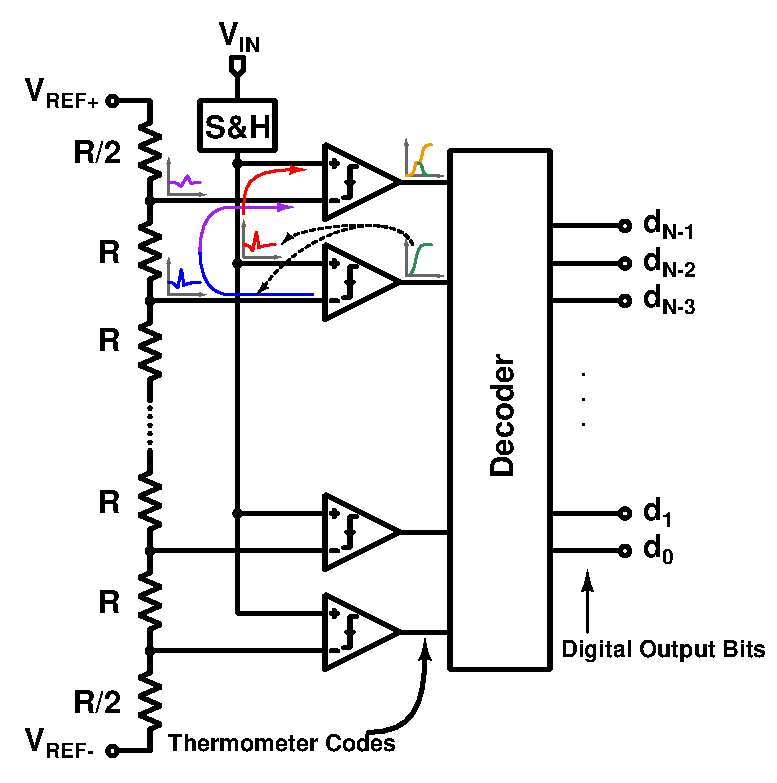
\includegraphics[height=8cm]{flash_adc.ps}
	\caption{comparators kickback noise impacts other comparator though the reference ladder}
	\label{fig:flash_kickback}
\end{figure}

Making fast decision the steep output voltage rise of a comparator engenders a glitch at the inputs of this one. This kickback noise propagates back to the reference ladder. This high impedance node introduce an offset between inputs. Comparators alongside are perturbed and could be falsely tripped.

As a results, the comparator outputs can likely be 001011 instead of 001111. The spurious zero among ones is caused by imperfect input settling. Moreover, comparators timing mismatch are also source of this bubble effect.

Area constraints as well as the sensitivity of this architecture limits the feasible resolution. The error of the conversion not being available, Flash ADC are not used in cascade to increase the overall resolution but are rather used in mixed converter or a the end of pipelined ADC\@.

%-- might add here a discussion on the thermal noise

%The following table gives as an abstract the main characteristics of these converters. It can be seen that most of them achieved very high speed and a low/medium resolution at the price of power consumption.

%-- add a table comparing some in literature

	\subsection{Folding}                           % section 2.1.2
	\label{sec:folding-adc}
In the Flash ADC, comparator gives the sign of differential voltages. The quantization can be viewed as a collection of zero crossings for references voltages scaling from 0 to \(V_{REF} \). Folding the signal as depicted by \figurename~\ref{fig:folding_principle} provides a component saving method. The number of components can be tremendously reduced. A folding amplifier generates the saw wave signal like the folding signal.

\begin{figure}[htp]
	\centering
	\resizebox{0.8\textwidth}{!} {\def\putbox#1#2#3#4{\makebox[0in][l]{\makebox[#1][l]{}\raisebox{\baselineskip}[0in][0in]{\raisebox{#2}[0in][0in]{\scalebox{#3}{#4}}}}}
\def\rightbox#1{\makebox[0in][r]{#1}}
\def\centbox#1{\makebox[0in]{#1}}
\def\topbox#1{\raisebox{-0.60\baselineskip}[0in][0in]{#1}}
\def\midbox#1{\raisebox{-0.20\baselineskip}[0in][0in]{#1}}
   \scalebox{1}{
   \normalsize
   \parbox{5.90104in}{
   \includegraphics[scale=1]{Chapter3/Figs/folding_signal_principle}\\
   % translate x=364 y=254 scale 0.38
   \putbox{1.70in}{0.09in}{1.20}{Input Voltage [V]}%
   \putbox{0.20in}{0.67in}{1.20}{\rotatebox{-270}{Voltage Processed [V]}}%
   \putbox{0.54in}{1.71in}{0.84}{\(V_{REF}\)}%
   \putbox{0.41in}{2.38in}{0.84}{3}%
   \putbox{0.66in}{1.50in}{0.84}{2}%
   \putbox{0.54in}{1.05in}{0.84}{\(V_{REF}\)}%
   \putbox{0.54in}{2.38in}{0.84}{\(V_{REF}\)}%
   \putbox{0.54in}{2.96in}{0.84}{\(V_{REF}\)}%
   \putbox{0.66in}{0.84in}{0.84}{4}%
   \putbox{0.58in}{2.17in}{0.84}{4}%
   } % close 'parbox'
   } % close 'scalebox'
   \vspace{-\baselineskip} % this is not necessary, but looks better
}
	\caption{Signal folding principle to reduce the number of needed comparators with a 5-bits example}
	\label{fig:folding_principle}
\end{figure}

The conversion is thus performed by two Flash ADC\@: one generates the Most-Significant-Bits (MSB) while the other performs a conversion of the folded signal. This reduces the total number of components relaxing previous constraints of Flash ADC~\cite{VanDePlassche1979, Grift1987, Nauta1995, Vorenkamp1997}. Unfortunately, the Folding Amplifier shall have a linearity greater than the fine Flash ADC and introduce several design constraints. Linearity can be corrected either by a digital calibration or by a resistive interpolation~\cite{Vorenkamp1997}.

\begin{figure}[htp]
	\centering
	\begin{subfigure}[b]{0.44\textwidth}
        \resizebox{\textwidth}{!}{% XCircuit output "folding_amplifier_parallel.tex" for LaTeX input from folding_amplifier_parallel.ps
\def\putbox#1#2#3#4{\makebox[0in][l]{\makebox[#1][l]{}\raisebox{\baselineskip}[0in][0in]{\raisebox{#2}[0in][0in]{\scalebox{#3}{#4}}}}}
\def\rightbox#1{\makebox[0in][r]{#1}}
\def\centbox#1{\makebox[0in]{#1}}
\def\topbox#1{\raisebox{-0.60\baselineskip}[0in][0in]{#1}}
\def\midbox#1{\raisebox{-0.20\baselineskip}[0in][0in]{#1}}
   \scalebox{1}{
   \normalsize
   \parbox{6.08333in}{
   \includegraphics[scale=1]{./folding_amplifier_parallel}\\
   % translate x=416 y=400 scale 0.38
   \putbox{3.72in}{1.39in}{2.40}{\ldots}%
   } % close 'parbox'
   } % close 'scalebox'
   \vspace{-\baselineskip} % this is not necessary, but looks better
}
        \subcaption{parallel}
        \label{fig:folding_amp_par}
    \end{subfigure}
    \begin{subfigure}[b]{0.52\textwidth}
        \resizebox{\textwidth}{!}{% XCircuit output "folding_amplifier_cascaded.tex" for LaTeX input from folding_amplifier_cascaded.ps
\def\putbox#1#2#3#4{\makebox[0in][l]{\makebox[#1][l]{}\raisebox{\baselineskip}[0in][0in]{\raisebox{#2}[0in][0in]{\scalebox{#3}{#4}}}}}
\def\rightbox#1{\makebox[0in][r]{#1}}
\def\centbox#1{\makebox[0in]{#1}}
\def\topbox#1{\raisebox{-0.60\baselineskip}[0in][0in]{#1}}
\def\midbox#1{\raisebox{-0.20\baselineskip}[0in][0in]{#1}}
   \scalebox{1}{
   \normalsize
   \parbox{8.27083in}{
   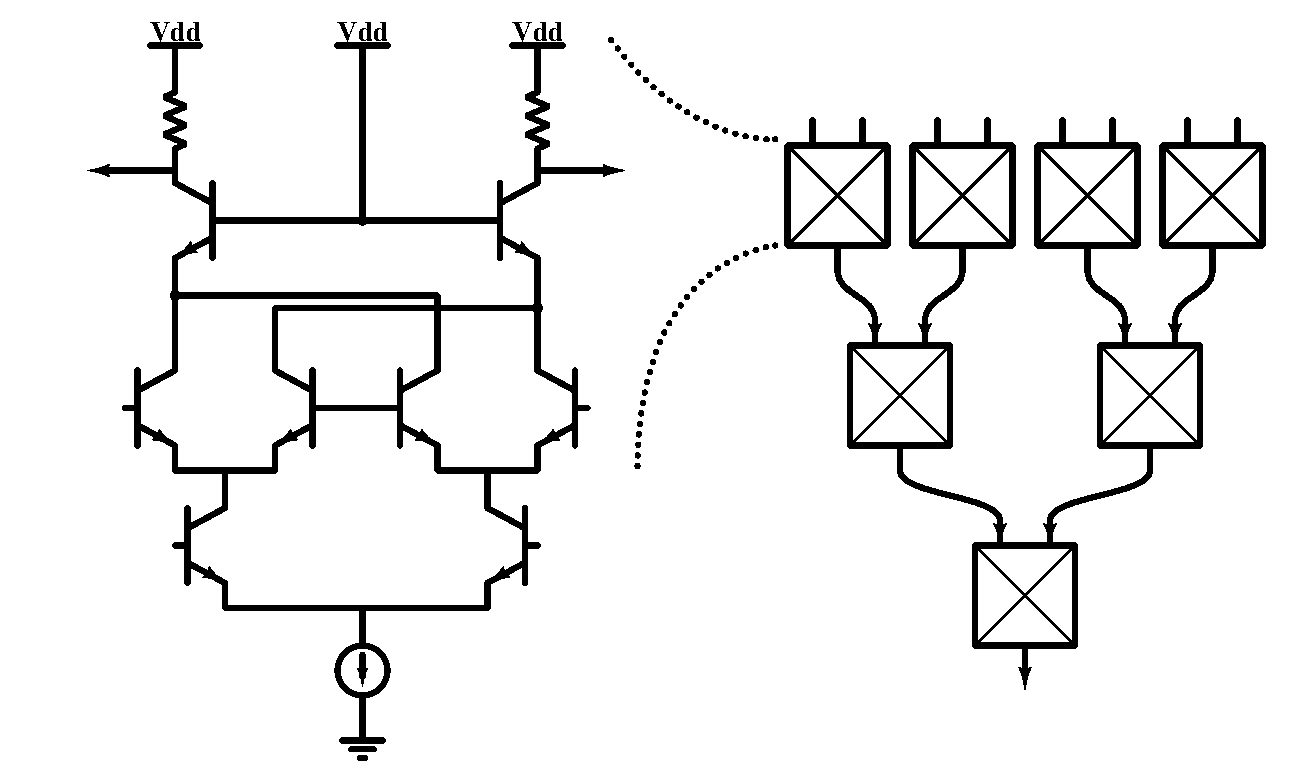
\includegraphics[scale=1]{./folding_amplifier_cascaded}\\
   % translate x=720 y=400 scale 0.38
   \putbox{0.81in}{1.39in}{1.20}{A}%
   \putbox{3.56in}{1.39in}{1.20}{An}%
   \putbox{3.89in}{2.31in}{1.20}{B}%
   \putbox{2.14in}{2.47in}{1.20}{Bn}%
   \putbox{0.47in}{2.31in}{1.20}{B}%
   \putbox{4.14in}{3.89in}{1.20}{\(V_{out+}\)}%
   \putbox{0.06in}{3.89in}{1.20}{\(V_{out-}\)}%
   \putbox{5.31in}{3.97in}{0.90}{A}%
   \putbox{5.56in}{3.97in}{0.90}{B}%
   \putbox{5.31in}{3.56in}{0.90}{OUT}%
   \putbox{6.14in}{3.97in}{0.90}{A}%
   \putbox{6.39in}{3.97in}{0.90}{B}%
   \putbox{6.14in}{3.56in}{0.90}{OUT}%
   \putbox{5.72in}{2.64in}{0.90}{A}%
   \putbox{5.97in}{2.64in}{0.90}{B}%
   \putbox{5.72in}{2.22in}{0.90}{OUT}%
   \putbox{6.97in}{3.97in}{0.90}{A}%
   \putbox{7.22in}{3.97in}{0.90}{B}%
   \putbox{6.97in}{3.56in}{0.90}{OUT}%
   \putbox{7.81in}{3.97in}{0.90}{A}%
   \putbox{8.06in}{3.97in}{0.90}{B}%
   \putbox{7.81in}{3.56in}{0.90}{OUT}%
   \putbox{7.39in}{2.64in}{0.90}{A}%
   \putbox{7.64in}{2.64in}{0.90}{B}%
   \putbox{7.39in}{2.22in}{0.90}{OUT}%
   \putbox{6.56in}{1.31in}{0.90}{A}%
   \putbox{6.81in}{1.31in}{0.90}{B}%
   \putbox{6.56in}{0.89in}{0.90}{OUT}%
   \putbox{5.22in}{4.39in}{1.20}{\(F_1\)}%
   \putbox{6.06in}{4.39in}{1.20}{\(F_2\)}%
   \putbox{5.56in}{4.39in}{1.20}{\(F_3\)}%
   \putbox{6.39in}{4.39in}{1.20}{\(F_4\)}%
   \putbox{6.81in}{4.39in}{1.20}{\(F_1D\)}%
   \putbox{7.64in}{4.39in}{1.20}{\(F_2D\)}%
   \putbox{7.14in}{4.39in}{1.20}{\(F_3D\)}%
   \putbox{7.97in}{4.39in}{1.20}{\(F_4D\)}%
   \putbox{6.51in}{0.39in}{1.20}{OUT}%
   } % close 'parbox'
   } % close 'scalebox'
   \vspace{-\baselineskip} % this is not necessary, but looks better
}
        \subcaption{cascade}
        \label{fig:folding_amp_casc}
    \end{subfigure}
	\caption{Folding amplifier implementation in a parallel fashion~\cite{Choe2001} and in a cascaded fashion~\cite{Vorenkamp1997}}
	\label{fig:folding_amplifier}
\end{figure}

The design of the folding amplifier as depicted by \figurename~\ref{fig:folding_amplifier} is sensitive to both the \(g_m\) mismatch of differential pairs and to tail current mismatch. These mismatches impact the zero crossings as an offset~\cite{Choe2001}, and interpolation is a way to mitigate this effect while increasing the resolution.

Such topology of ADC allows the cascade of several stages~\cite{Taft2009, Buck2017}, making a good candidate to achieve medium resolution at high speed~\cite{Vorenkamp1997, Pan2000}. The biggest flaws of Folding Architecture is the area and the power consumption despite works to reduce them~\cite{Costa2013}.

The comparison table~\ref{table:folding_comparison_table} stresses out the bump in resolution such architecture provide over Flash ADC\@. They achieve a very high speed with a slightly increased latency. This can ve viewed as a trade of time for resolution.

\begin{table}[htp]
	\caption{Folding ADC in the literature}
	\centering
	\label{table:folding_comparison_table}
	\begin{tabular}{L{3.5\charwidth} C{23\charwidth} R{6.5\charwidth} R{4\charwidth} S[table-format=2.2, table-column-width=5.2\charwidth] R{6\charwidth} R{5.5\charwidth} R{3.5\charwidth}}
		\toprule
	Ref. & Architecture & Techno. [nm] & \(F_{snyq}\) [MHz] & {\makecell{{Area}\\{[\(mm^2 \)]}}} & Supply [V] & Power [mW] & Res. \tabularnewline \midrule
	\cite{Vorenkamp1997} & Folding \& Interpolation  & 1000 &   60 &    7 &   5 &  300 & 12 \\
	\cite{Choe2001}      & Folding                   &  500 &  100 & 1.68 &   5 &  165 &  8 \\
	\cite{Taft2009}      & Cascaded Folding          &  180 & 1000 &   49 & 1.8 & 1260 & 10 \\
	\cite{Buck2017}      & Folding \& Interpolation  &  250 & 6000 & 13.3 & 5.1/3 & 10200 & 10 \\
	\cite{Costa2013}     & switched-cap Folding      &  350 &  100 &   NA & 3.3 &  2.5 &  8 \\
	\bottomrule
	\end{tabular}
\end{table}
\nomenclature[A-Fsnyq]{$F_{snyq}$}{nyquist frequency}

\subsection{Successive Approximation Register} % section 2.1.3
\label{sec:sar-adc}
\nomenclature[z]{SAR}{Successive Approximation Register}
The first appearance of SAR ARC was back in early 70s~\cite{McCreary1975}. Using a binary search algorithm, this kind of converter is by far slower than a Flash or Folding ADC\@. As represented in \figurename~\ref{fig:sar_adc}, the SAR does not have any active component such an amplifier making it very efficient and targeting low-power application. But they are also able to performs either high-resolution conversions or high-speed conversions.

\begin{figure}[htp]
	\centering
	\begin{subfigure}[b]{0.44\textwidth}
        \includegraphics[width=\textwidth]{sar_principle.ps}
        \subcaption{principle}
        \label{fig:sar_principle}
    \end{subfigure}
    \begin{subfigure}[b]{0.52\textwidth}
        \includegraphics[width=\textwidth]{sar_classic_dac.ps}
        \subcaption{traditional DAC implementation}
        \label{fig:sar_dac_classical}
    \end{subfigure}
	\caption{traditional charge redistribution SAR ADC as presented in~\cite{McCreary1975}}
	\label{fig:sar_adc}
\end{figure}

The architecture also benefits from using only one comparator to reduce the occupied area. With recent progress, the SAR converter outperformed power consumption, its area occupancy have been tremendously shrink, and the speed have been soared. The primary source of power dissipation are the digital control circuit, the comparator, and capacitive reference DAC network. The advancement in technology also favours the speed of the digital logic while the power consumption of the comparator and the capacitive DAC is limited by mismatch and noise~\cite{Yue2013,Mueller2013,Collins2017}. To address both the area occupancy and further reduce the energy consumption, the DAC architecture can be optimized by decreasing the capacitance and still preserving the binary scale.
\nomenclature[z]{ADC}{Analog-to-Digital Converter}
\nomenclature[z]{DAC}{Digital-to-Analog Converter}

%\subsubsection{architecture}	
Having high resolution SAR ADC is quite challenging. Using a binary weighted capacitive reference in the DAC network leads to a increasing number of capacitors. Stereotypical capacitive DAC forms a binary scale split into a bunch of unit capacitors, so that the n-th capacitor in the scale is a group of \(2^N\) of them. To increase the resolution from N to N+1, we add \(2^{N+1}\) unit capacitors. Thus the occupied area grows exponentially as the resolution increased. And considering a differential structure, the phenomenon is even more pronounced causing lateral effects such as an excessive reference voltage loading.

Conventional techniques to shrink the area and to relax constraints on voltage buffers, designers usually play with serial-parallel configurations of unit components. This results into well known techniques called split-junction and split-capacitor. 

The split-capacitor as represented in \figurename~\ref{fig:split_capacitor} inserts a capacitor which scale down a segment of the DAC\@. Thus, bigger capacitor can be sized down to preserve the scale. The diminution of load provides substantial power savings. The implementation obstacle is introduced by the attenuation capacitor not being a multiple integer of the unit capacitor. Moreover, an extra switch par segmented DAC is introduced for the sampling of the input signal. Thus, the thermal noise is increased by both the scale down of capacitance and by the extra noise source switches represents.

\begin{figure}[htp]
	\centering
	\begin{subfigure}[b]{0.46\textwidth}
        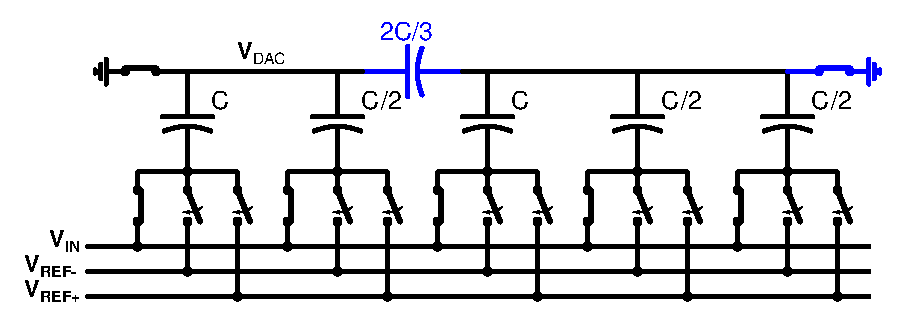
\includegraphics[width=\textwidth]{sar_split_cap_dac.ps}
        \subcaption{split capacitor}
        \label{fig:split_capacitor}
    \end{subfigure}
    \begin{subfigure}[b]{0.52\textwidth}
        \includegraphics[width=\textwidth]{sar_split_junction_dac.ps}
        \subcaption{split junction}
        \label{fig:split_junction}
    \end{subfigure}
	\caption{DAC optimization by altering capacitors connections}
	\label{fig:sar_split_dac}
\end{figure}

However, capacitor can be connected in parallel as in \figurename~\ref{fig:split_junction}. Introduced in~\cite{Lee2008} and optimized in~\cite{Yu2010}, the split junction scheme has a superior efficiency by reducing the number of ``down'' transition by appending extra section in parallel to redistribute charges. The two-step junction-splitting capacitor array requires more switches than the conventional and junction-splitting ones, but reduces the total capacitance by a factor \(2^{N/2}\). From a thermal point of view, this architecture is more sensitive to thermal noise by adding noise source on the floating node \(V_{DAC}\). The floating node connected on the comparator inputs leads to excessive decision error at high temperatures. Such error could be mitigated with the help of redundancy and non binary ratio of the DAC scale~\cite{Zhang2014}.

%\subsubsection{switching method}
	\label{sec:sar-switching}
The low-power asset of the SAR ADC can further be improved by a careful attention of switching energy loss. The conventional charge-redistribution method is not power effective~\cite{Ginsburg2005} owing to the discharge of the capacitor weight under test and charging-back this capacitor. Even if lot of progress comes by a load reduction as discussed previously, the switching can strikingly reduce the power consumption; as far as 98\% of the conventional switching scheme~\cite{Zhu2013,Xie2014,Li2016}.
The first technique which draws attention was the monotonic switching. Since the first clock cycle are the more power hungry, the monotonic switching sample the differential input voltage on the top-plates of capacitors while the common-mode voltage \(V_{cm}\) is applied on the bottom-plates. As represented in \figurename~\ref{fig:sar_vcm_monotonic}, the comparator determine first bit \(d_0\) as polarity of the differential voltage~\cite{Ginsburg2005}. Compared to the conventional switching method, the reset of the MSB capacitor is saved. Moreover, a N-1 bits DAC is sufficient to output N-bits. Then, According to the comparison results, the logic unit will connect the largest capacitor of bigger voltage side to the ground, and the other side remains the same. Therefore almost half of the switching energy is saved. However, the common-mode level is decreasing during the monotonic switching, which puts a high demand on the performance of the comparator.

\begin{figure}[htp]
	\centering
	\includegraphics[width=0.8\textwidth]{sar_vcm_monotonic.ps}
	\caption{\(V_{cm}\)-based monotonic digital switching to reduce area and save switching energy}
	\label{fig:sar_vcm_monotonic}
\end{figure}

Moreover, the switching loss is voltage dependent. The reduction of the voltage step diminishes the switching loss in the same proportion. Using  \(V_{cm}\) instead of the ground already halves the switching energy. Thus, in the sampling phase, the differential input is sampled as inputs on the top-plates (\(V_{DAC}\)) while the bottom-plates is connected to \(V_{cm}\). After the sampling phase, during each conversion cycle of a \(V_{cm}\)-based switching, the bottom plates of the capacitors will be switched in descending order, from \(V_{cm}\) to \(V_{refp}\) in one-side or another depending on each bit decision as depicted by \figurename~\ref{fig:sar_vcm_monotonic}. The connection to \(V_{cm}\) adds one switch per capacitor increasing the thermal noise sources.

The switching being optimized a further improvement could come from an assumption on the signal converted. As sensors outputs react slowly and their voltage are usually filtered in front, the input signal of the ADC is of low mean activity over a time window. The conversion can start from an initial guess which is the output of the previous sample~\cite{Yaul2014}. Bit-cycling only last bits, the LSB first conversion performed is power efficient. When the error between the final code and the initial guess overtake few LSB, a complete conversion shall be performed. Therefore, the power savings is inherent to the nature of the input signal. Without such assumption, the power consumption is higher than previous methods and limit the speed of the conversion.

%\subsubsection{digital implementation}
Once the analog and the switching optimized, the remaining part to optimize is the digital. The clock rate deeply linked to the power consumption enters in conflict of specification for manufacturable design: The internal clock limit the settling time of DAC and the decision time of the comparator. Taking into account process voltage temperature variation, it is usual to base the sampling frequency on the peak delay in the worst corner. Compared with synchronous design, using asynchronous logic could relax constraints on the comparator design. The conversion time \(T_{conv}  \) shall respect at least the following inequality
\begin{equation}
\label{eqn:sar_async_conv}
%\vcenter{\hbox{\includegraphics[width=0.45\textwidth]{sar_principle_timing.ps}}}
T_{conv} >= \sum_{i=0}^N {\textcolor{blue}{t_{cmp, i}}+\textcolor{red}{T_{Logic, i}}+\textcolor{Xgreen}{t_{DAC, i}}}
\end{equation}
where \(t_{cmp, i}\) is the delay of the comparator, \(T_{Logic, i}\) the propagation time of the logic toggling switches, \(t_{DAC, i}\) the settling time of the DAC\@.

In a synchronous SAR, the two clock phase are used such that the first phase is dedicated to the DAC settling and the reset of the comparator whereas the second phase is devoted to the comparator decision and finish the settling.

In an asynchronous SAR, the digital logic should control when the comparator reset and the moment to make a decision. With regard to the logic, a delay larger than the total delay from comparator to the switching signals shall be ensured between the ready signal and the new decision start~\cite{Brenna2014}. By using a single XOR or NAND gate of the comparator outputs, a ready (valid) signal can be asserted~\cite{Brenna2014, Sekimoto2011, Zhu2015,Shen2018}. In turns, the ready signal trigger the reset of the comparator and the DAC settling. A delayed copy of the ready signal starts a new decision. This solution based on standard cells still require delay cells. The delay sensitive to PVT variation, an asynchronous control is preferred. As done in \figurename~\ref{fig:sar_logic_jchen2011}~\cite{JChen2011}, two loops can control respectively the reset and the next decision latching. Unfortunately, the double-input T-flip-flop is not among standard cells in many process. Moreover, the loop of the reset (in blue) should be ensured to be faster than the loop of the set (in red) over PVT variations after place and route. S.S. Wong \textit{et al.} presented switching signals to trigger the asynchronous loop instead of a fixed delay of comparator ready signal or asynchronous loop~\cite{Wong2013}. The process variation problem caused by the control logic and buffers is thus overcome without any tunable or worst case delay cells. Represented in \figurename~\ref{fig:sar_logic_wong2013}, this also has the benefit of more easily ensure that DAC settling is started before triggering the comparator.

\begin{figure}[htp]
	\centering
	%\begin{subfigure}[b]{0.29\textwidth}
    %    \includegraphics[width=\textwidth]{sar_logic_Shen2018.ps}
    %    \subcaption{standard clock generation}
    %    \label{fig:sar_logic_basic}
    %\end{subfigure}
    \begin{subfigure}[b]{0.48\textwidth}
        \includegraphics[width=\textwidth]{sar_logic_JChen2011.ps}
        \subcaption{seperate clock/reset loop}
        \label{fig:sar_logic_jchen2011}
	\end{subfigure}
	\begin{subfigure}[b]{0.44\textwidth}
        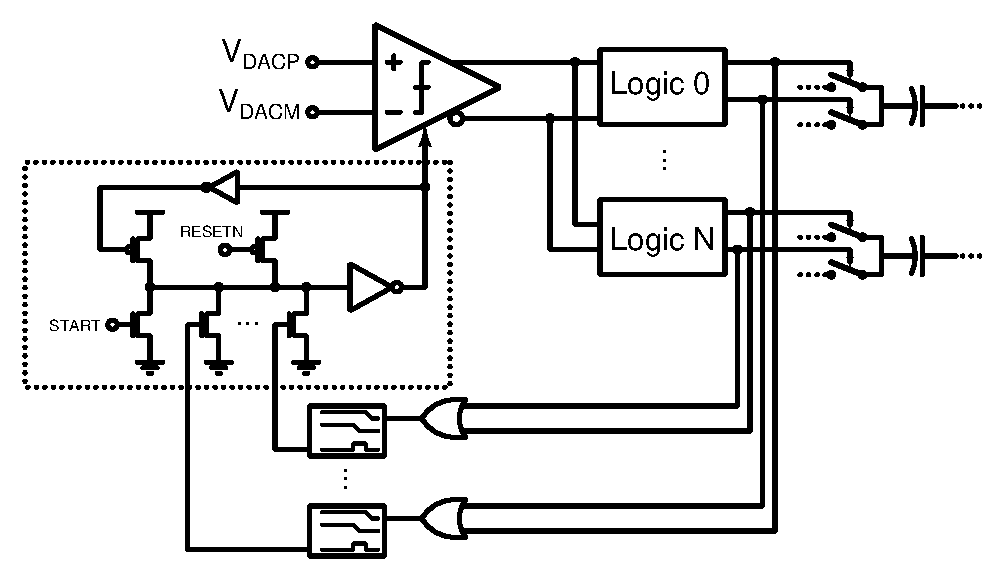
\includegraphics[width=\textwidth]{sar_logic_wong2013.ps}
        \subcaption{clock generation in~\cite{Wong2013}}
        \label{fig:sar_logic_wong2013}
    \end{subfigure}
	\caption{comparator's clock generation}
	\label{fig:sar_cmp_clock}
\end{figure}

In addition, when the input voltages of the comparator are closer to each other, the comparator decision in either way to zero or one lasts longer. At low-temperature when the noise is not sufficient to force the latch in a state, metastability is inevitable. For unusually too long decision time, the digital code might be incomplete and results in errors. In~\cite{Tung2016} a timer circuit provide a timing slot which at the end a flag is raised to indicate the metastability and force the execution of subsequent cycles.

Moreover, the PVT variation alters the settling of the DAC\@. Instead of waiting the full settling and sizing accordingly delay cells,~\cite{Kull2013} suggests that decision errors due to a partial settling can be tolerated with redundancy. An erroneous decision in the redundant region, via the non-binary scale of the DAC, is corrected by a latter decision.

In~\cite{Brenna2014, Shen2018} the SAR logic implement a shift register cadenced by ready (valid) signal and generate the end of conversion flag for the asynchronous clock generator. To the contrary,~\cite{Wong2013} waits the ready (valid) signal of the LSB logic.
\nomenclature[z]{MSB}{Most Significant Bit}
\nomenclature[z]{LSB}{Least Significant Bit}

The table~\ref{table:sar_comparison_table} gives as an abstract the main characteristics of these converters. It can be seen that most of them achieved high speed and a low/medium resolution with fairly small power consumption.

\begin{table}[htp]
	\caption{SAR ADC in the literature}
	\centering
	\label{table:sar_comparison_table}
	\begin{tabular}{L{3.5\charwidth} C{23\charwidth} R{6.5\charwidth} R{4\charwidth} S[table-format=2.2, table-column-width=5.2\charwidth] R{6\charwidth} R{5.5\charwidth} R{3.5\charwidth}}
	\toprule
	Ref. & Architecture & Techno. [nm] & \(F_{snyq}\) [MHz] & {\makecell{{Area}\\{[\(mm^2\)]}}} & Supply [V] & Power [\(\mu \)W] & Res. \tabularnewline \midrule
	\cite{Zhang2014} & 1.85-radix classic~CDAC   &  65 &  10 & 0.01 &  NA &   50 & 15 \\
	\cite{Shen2018}  & classic~CDAC asynchronous & 180 &  20 & 1.61 & 1.8 & 1770 & 12 \\
	\cite{Zhu2010}   & split-cap Vcm-based       &  90 & 100 & 0.18 & 1.2 & 3000 & 10 \\
	\cite{Liu2010}   & classic~CDAC Monotonic    & 130 &  50 & 0.05 & 1.2 &  826 & 10 \\
	\cite{Harpe2011} & classic~CDAC asynchronous &  90 &  10 & 0.05 &   1 &   26 &  8 \\
	\bottomrule
	\end{tabular}
\end{table}


	\subsection{\(\Delta\Sigma \) Converters}      % section 2.1.4
	\label{sec:sd-isd-adc}
DELTA-SIGMA (\(\Delta\Sigma \)) modulation efficiently performs high-resolution data conversion using oversampling. The	implementation imperfections including matching errors and offsets which limit the obtainable resolution of Nyquist rate converters can thus be surmounted. With increasing bandwidth demands, reducing the oversampling ratio (OSR) is important to meet the required input bandwidth while also attaining medium to high resolution as expected from oversampled converters. 
\nomenclature[z]{OSR}{Oversampling Ratio}

Further improvements can be achieved by the increase of the noise shaping order. The improve originates from extra integrator in the forward path. Unfortunately feedback structure of the modulator is prone to instability for hig-order of noise shaping (>= 3). Additionally, high-order modulators suffer from a stability dependence on system parameters such as integrator gains and delays, input amplitude, transients, initial conditions, or even saturation limit cycles~\cite{Hein1993,Baird1994,Steven1996}. The dominant means of stabilizing high-order systems is identified to be the use of multi-bit quantization since this transforms the nature of the system rather than just restricting the region of operation. However, the cumbersome implementation of the multi-level error feedback DACs can significantly reduce the modulator performance for a not extremely linear one~\cite{Medeiro1999}. 

To the opposite, first-order modulators are inherently stable. A cascade of such modulator results in an increased noise shaping order without the stability issue or sacrificing the input amplitude~\cite{Brooks1997}. Their advantage is that no individual modulator needs to be designed with a high-order filter; the total filter order can be spread out across many different stages so that each individual \(\Delta\Sigma \) stage will only be of low order. The modulator stability will be a function of the individual lower order modulators rather than the total order of the modulator.

The digital output of individual \(\Delta\Sigma \) modulators is then processed by a digital filter. It is designed to reduce error introduced in first stages by the product of the Noise-Transfer-Function of each stage. This cancellation is dependent on matching between the digital filters and the analog filters within modulators. The latter is one of the major limitations for high-resolution cascaded \(\Delta\Sigma \) modulators leveraged by digital calibration~\cite{Cauwenberghs2000}.

Unlike conventional \(\Delta\Sigma \) ADC, the analog loop filter and digital filter in Incremental-\(\Delta\Sigma \) (\(I\Delta\Sigma \)) ADC are reset after oversampling each input sample. As a result, \(I\Delta\Sigma \) ADC can offer sample-by-sample conversion much like Nyquist-rate ADC allowing multiplexing of different inputs to be done without cross talk. Additionally, comparing to ultra-low-power SAR ADC, which feature medium-resolution, \(I\Delta\Sigma \) ADC relax the requirements of the analog front-end (AFE) circuitry: the variable-gain amplifier (VGA) can be eliminated, and the active anti-aliasing filter (AAF) can be replaced by a passive filter.

\begin{figure}[htp]
	\centering
	\resizebox{\textwidth}{!} {\def\putbox#1#2#3#4{\makebox[0in][l]{\makebox[#1][l]{}\raisebox{\baselineskip}[0in][0in]{\raisebox{#2}[0in][0in]{\scalebox{#3}{#4}}}}}
\def\rightbox#1{\makebox[0in][r]{#1}}
\def\centbox#1{\makebox[0in]{#1}}
\def\topbox#1{\raisebox{-0.60\baselineskip}[0in][0in]{#1}}
\def\midbox#1{\raisebox{-0.20\baselineskip}[0in][0in]{#1}}
   \scalebox{1}{
   \normalsize
   \parbox{7.08333in}{
   \includegraphics[scale=1]{Chapter3/Figs/isd_first_order_principle}\\
   % translate x=568 y=192 scale 0.38
   \putbox{0.81in}{0.68in}{0.90}{S/H}%
   \putbox{2.14in}{0.56in}{0.90}{$\Phi_r$}%
   \putbox{2.76in}{0.76in}{0.96}{1}%
   \putbox{2.68in}{0.56in}{0.96}{Z-1}%
   \putbox{3.85in}{0.68in}{0.90}{A/D}%
   \putbox{3.85in}{0.18in}{0.90}{D/A}%
   \putbox{4.47in}{0.56in}{0.90}{$\Phi_r$}%
   \putbox{5.10in}{0.76in}{0.96}{1}%
   \putbox{5.01in}{0.56in}{0.96}{Z-1}%
   \putbox{4.35in}{0.85in}{1.20}{$d_k$}%
   \putbox{0.06in}{0.68in}{1.20}{$V_{in}$}%
   \putbox{6.81in}{0.68in}{1.20}{$D_{out}$}%
   \putbox{6.18in}{0.68in}{0.90}{M}%
   } % close 'parbox'
   } % close 'scalebox'
   \vspace{-\baselineskip} % this is not necessary, but looks better
}
	\caption{First Order Incremental-\(\Delta\Sigma \)}
	\label{fig:isd_first_order_principle}
\end{figure}

A first order \(I\Delta\Sigma \) as represented in \figurename~\ref{fig:isd_first_order_principle} a resolution of N-bits is achieved in \(2^N \) clock cycle. Different approaches have been proposed to significantly enhance the conversion speed and/or resolution of \(I\Delta\Sigma \) ADC~\cite{Markus2004,Quiquempoix2006,Caldwell2010}. The most popular alternatives are high-order architectures~\cite{Au1997,Babanezhad1991,Baird1996}. Other alternatives are the extended counting (EC-ADC)~\cite{Jeon2017,Baird1995,Chen2016} and the extended range (ER-ADC)~\cite{Agah2010,Rossi2009} architectures, which combine the \(I\Delta\Sigma \) ADC with a low-power Nyquist-rate ADC\@. The main difference between the two is that in an EC-ADC, the \(I\Delta\Sigma \) ADC hardware is usually reused and reconfigured as a cyclic ADC, while in an ER-ADC, the residue  of the \(I\Delta\Sigma \) is processed by another Nyquist-rate ADC\@. Recent advances in \(I\Delta\Sigma \) ADC showcase further improvement in power efficiency by employing inverter-based integrators~\cite{Chae2009}, or comparator based integrators~\cite{Yamamoto2012}.

An added benefit to \(I\Delta\Sigma \) is the simplicity of the decimation filter: the input signal is reconstituted as the mean value of the output bits for a first order while for higher order the representation of the input signal is given by a weighted multiple integral. For a third order \(V_{in}\) is estimated by the equation~(\ref{eqn:isd-decimation}).

\begin{equation}
	\frac{V_{\rm in}}{V_{\rm ref}}\approx \frac{3!}{(n-2)(n-1)n}\sum_{m=0}^{n-1}\sum_{l=0}^{m-1}\sum_{k=0}^{l-1}d_{k}
\label{eqn:isd-decimation}
\end{equation}

In~\cite{Caldwell2010} the number of output level for an \(L^{th}\)-order converter with \(N\) quantizer levels and an OSR of \(M\) is 
\begin{equation}
	\alpha(N-1)\frac{(M+L-1)!}{L!(M-1)!}+1
\label{eqn:isd-levels}
\end{equation}

The coefficient \(\alpha \) is the maximum converter amplitude that keeps the quantizer input bounded and is usually less than unity. The Signal-to-Noise Ratio (SNR) is thus defined as \(SNR = 6.02N + 1.76dB\). In other term, the input-referred noise of an Incremental-\(\Delta\Sigma \) comes from a weight association of each sample, and for higher order modulators earlier samples have a higher weighting than later samples because the digital filter has non-uniform weighting coefficients for higher order modulators. The equation~(\ref{eqn:isd_noise}) expresses the total input-referred noise power \(\overline{v_{n}^{2}}\)
\nomenclature[z]{SNR}{Signal over Noise Ratio}
\begin{equation}
	\overline{v_{n}^{2}}=\sum_{i=1}^{M}w_{i}^{2}\overline{v_{s}^{2}}=\overline{v_{s}^{2}}\sum_{i=1}^{M}w_{i}^{2}
\label{eqn:isd_noise}
\end{equation}
where \(\overline{v_{s}^{2}}\) is the input noise power of each sample, \(M\) is the OSR, and \(w_i\) is the weight associated with each sample.
\nomenclature[C-comp]{$\overline{X}$}{complementary of signal X}

In a first-order modulator, and assuming an accumulator as a decimation filter, the output as an average of the M inputs added to the quantization noise error introduced leads to \(w_i=1/M\). The resulting input-referred noise power is \(\overline{v_{n}^{2}}/M\), as expected for an ADC oversampled by M.

Nevertheless, in low-osr architecture a clock cycle is dedicated to the reset of the integrator which limits the resolution. The table~\ref{table:sigma_delta_comparison_table} compares \(I\Delta\Sigma \) to highlight the main characteristics of these converters. 

\begin{table}[htp]
	\caption{\(I\Delta\Sigma \)-ADC in the literature}
	\centering
	\label{table:sigma_delta_comparison_table}
	\begin{tabular}{L{3.5\charwidth} R{16.5\charwidth} R{6\charwidth} C{5\charwidth} R{4\charwidth} S[table-format=2.2, table-column-width=6\charwidth] R{6\charwidth} S[table-format=2.2, table-column-width=6\charwidth] C{3.5\charwidth}}
	\toprule
	Ref. & Architecture & Techno. [nm] & \(F_{snyq}\) [kHz] & OSR & {\makecell{{Area}\\{[\(mm^2 \)]}}} & Supply [V] & {\makecell{{Power}\\{[mW]}}} & Res. \\ 
	\midrule
	\cite{Quiquempoix2006} & \(3^{rd}\) Order \(I\Delta\Sigma \) & 600 & 30.72 & 512 & 2.08 & 2.5/5 & 0.6 & 22 \\
	\cite{Chae2009} & \(3^{rd}\) Order \(\Delta\Sigma \) & 180 & 40 & 100 & 0.715 & 0.7 & 0.036 & 14 \\
	\cite{Jeon2017} & EC-\(\Delta\Sigma \) & 180 & 185 & 8 & 0.0069 & 1.8 & 0.022 & 12 \\
	\cite{Agah2010} & ER-\(I\Delta\Sigma \) & 180 & 1000 & 45 & 3.5 & 1.8 & 38.1 & 14 \\
	\cite{Liu2017} & 1-1-1~MASH CT-\(\Delta\Sigma \) & 40 & 50000 & 29.7 & 0.177 & 1.2/2.5 & 19.7 & 11 \\
	\bottomrule
	\end{tabular}
\end{table}

	\subsection{Pipelined and Algorithmic}               % section 2.1.5 
	\label{sec:pipe-adc}
Low-voltage ADC have garnered much attention recently~\cite{Steyaert2012,Lee2011,SKLee2011,Brooks2009,Hershberg2012,YLim2015,YLim2015FD,Megawer2016,YCao2017}. This trend is a result of technology scaling as well as power efficiency associated with low-voltage circuits. Systems that inherently require low-voltage operation, such as
biomedical and wireless sensor applications, also motivate research in this area~\cite{Steyaert2012,Lee2011,SKLee2011}.

As depicted by the \figurename~\ref{fig:algo_principle} in a N-bit/cycle version, the input voltage \(V_{IN}\) is first sampled. The quadrant in which is the input voltage is determine by a N-bit sub-ADC\@. Then, the subtraction of the quadrant equivalent voltage centers the input voltage to be scaled by \(A\). In an pipelined ADC, another analog processing element receive this generated voltage as its input. In an algorithmic ADC, the new input voltage is the results of this analog process. In other term, the analog recycle an amplification of the error between the original input voltage and its successive rough estimation.
For a gain \(A=2\), the algorithmic ADC perform a modified binary search algorithm to digitize the input voltage. In this regard, the conversion is similar to SAR ADC with the fact that it provides the error of conversion\@.

\begin{figure}[htp]
	\centering
    \begin{subfigure}[b]{0.5\textwidth}
        \includegraphics[width=\textwidth]{algorithmic_principle.ps}
        \subcaption{principle}
        \label{fig:algo_principle}
	\end{subfigure}
	\begin{subfigure}[b]{0.48\textwidth}
        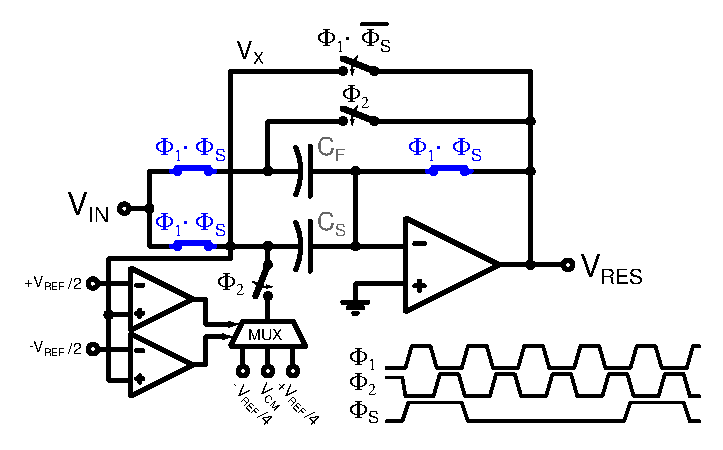
\includegraphics[width=\textwidth]{algo_mdac_std.ps}
        \subcaption{typical MDAC implementation}
        \label{fig:algo_mdac}
    \end{subfigure}
	\caption{principle of the algorithmic amplifier}
	\label{fig:algo_desc}
\end{figure}

As basic current mode method offers an ease of implementation of basic functions such as summation and scaling, they are also appropriate for low voltage application. Furthermore, current method fits high speed circuit specification. Therefore, current mode algorithmic have been designed~\cite{Nairn1990,Wang1991,Khodabndehloo2009,Bhatia2011}. Even if current mode design require lower voltage swing and increase noise immunity, the accuracy is limited by current mirror matching of the process. This can be
improved by increasing transistor sizes and biasing currents. Larger transistor sizes and larger reference current, however, need larger chip area, cost more, lower conversion speed, and increase power consumption, and in turn may make the proposed Current Mode ADC less attractive than other types of ADCs\cite{Wang1991}. Over very large temperature range, the design inevitably undergoes a tremendous performance drop while the mismatch of current of transistors is merely controlled over temperature~\cite{Shoucair1989, Andricciola2009}.

A common implementation of the algorithmic converter is by building the stage around a Flip-Around Multiplying DAC (FA-MDAC). This way, the closed-loop gain is defined by a ratio of capacitor whose mismatch is well controlled, as represented in \figurename~\ref{fig:algo_mdac}. \nomenclature[z]{MDAC}{Multiplying Digital-to-Analog Converter}

A simple differential pair is a valid amplifier to operate under low-supply condition. As the resolution increased (recycling of its inner self error), the gain of the amplifier shall drastically increase. By stacking transistors the output swing is thus limited: and non-linearity occurs. Therefore, medium to high resolution algorithmic ADC require a digital compensation~\cite{Murmann2003} or an adjustment of its residue curve~\cite{Inoue2017,Naderi2017}.

		\subsubsection{Comparator based}
To overcome the limitation of a traditional amplifier, a comparator driving current source/sinks can advantageously emulate one. While amplifier tries to continuously force its inputs to be virtual ground, in comparator based switched capacitor (CBSC) circuit, virtual ground is detect by a comparator which stops to pressure on the inputs.

\begin{figure}[htp]
	\centering
	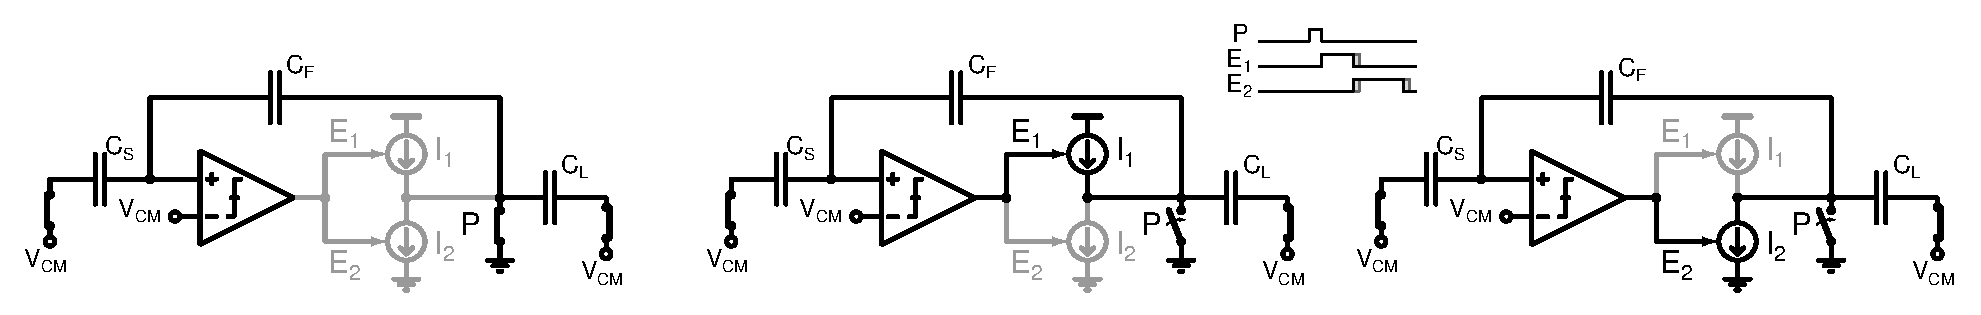
\includegraphics[width=\textwidth]{algo_comp_based.ps}
	\caption{Comparator Based charge transfer}
	\label{fig:algo_comp_based}
\end{figure}

\figurename~\ref{fig:algo_comp_based} represents how does the charges are transferred. The comparator inputs should be first shifted from their virtual ground condition to start a new transfer. In a second phase, the a large current ramp the output voltage in a similar way an amplifier slewing does. When the virtual ground is detected, the current source is turned off. Due to comparator's delay, an overshoot occurs. In third phase, a small current of opposite sign reverts the overshoot and get a more accurate measurement of the virtual ground condition turning off the second current source. This is similar to the linear behaviour of an amplifier.

The accuracy of the settling is thus limited by the comparator's offset, the comparator resolution, the delay of the comparator, the slewing, the digital phase variations, and the noise in the third accurate phase~\cite{Fiorenza2006}.
Folded flicker noise was found to be a significant contributor to the broadband noise: because the flicker noise of the comparator extends beyond the Nyquist rate of the converter~\cite{Sepke2008}. However, they exhibit less inherent noise than a traditional amplifier in a switched capacitor circuit~\cite{Fiorenza2006}.

In~\cite{Brooks2009}, a fully differential version have been proposed. Sensitive to current mismatch of process variation, this structure introduce as an extra offset not compensated worsen by the temperature. A chopper stabilization~\cite{Toth2003} and their alternatives can still be used to correct the introduced offset~\cite{Brooks2009}.
Thence the limitation of the overshoot can be leveraged by ramping in only one direction~\cite{Lee2012}. This architecture blend power consumption, high speed even for very low power supply~\cite{Steyaert2012}.

		\subsubsection{Ring Amplifier based}
The digital phases being cumbersome, another amplifier emulation have been proposed: the Ring Amplifier. The Ring Amplifier is a three-stage inverter-based structure that have a large output swing, and its slew-based charging characterization makes it able to charge large capacitive load efficiently~\cite{Hershberg2012}.
In closed loop configuration, the odd numbered stage structure is oscillating. A dead zone defined by design, kill the oscillation in a small zone around the trip point of the first inverter.
The design of an accurate ring amplifier implies a tiny dead zone a few microvolts wherein output transistors are in sub-threshold. At the edge of the stability zone, and taking into consideration PVT variations, the dead zone is practically few millivolts. Despite this, it is found in several high speed, high accuracy ADC~\cite{Hershberg2012,YLim2015,YLim2015FD,YCao2017}.

The first improvement over~\cite{Hershberg2012} is found in~\cite{YLim2015} where the biasing is self-generated by an IR drop in the middle stage. The IR drop is realized by a resistance of few kilo-Ohms. Moreover, the final stage use high threshold voltage transistor to further improves the stability by increasing the dead zone. Unfortunately, the speed, the accuracy, and the stability is tightly coupled with the self-biasing resistance introduced.

\begin{figure}[htp]
	\centering
    \begin{subfigure}[b]{0.5\textwidth}
        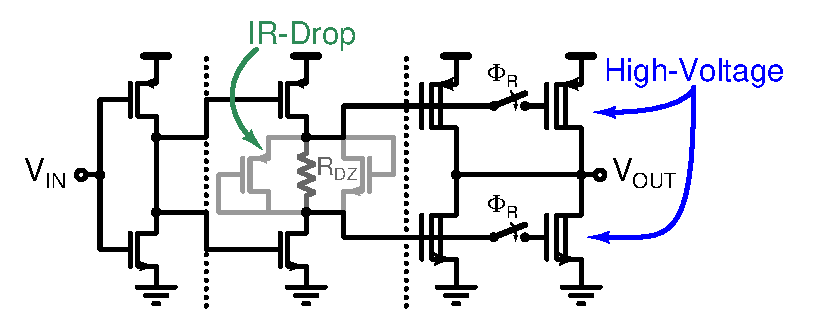
\includegraphics[width=\textwidth]{ring_amplifier_variations.ps}
		\subcaption{variations}
        \label{fig:ring_amp_variation}
	\end{subfigure}
	\begin{subfigure}[b]{0.48\textwidth}
        \includegraphics[width=\textwidth]{fully_diff_ring_amp.ps}
        \subcaption{Fully-Differential Version}
        \label{fig:ring_amp_fd}
    \end{subfigure}
	\caption[Ring Amplifier common variations]{Ring Amplifier common variations as in~\cite{YLim2015,YLim2015FD,YCao2017}}
	\label{fig:algo_ring_amp}
\end{figure}

To improve the accuracy~\cite{Megawer2016} adds an auto-zero phase in which the complete ring amplifier is reset (shunt). Both the input offset and output offset are thus ``trimmed''. To counter the fact that a reset of the fully ring amplifier generates a ring oscillator. The dead zone is thus enlarge to cut the oscillation path. To improve the efficiency, the final stage is changed to have a different slewing in the amplification phase and in the auto-zero phase. Sacrificing the speed by increasing the IR drop resistance, the IR drop is then changed into a common resistor for both amplification and auto-zero phase with an extra resistor for the auto-zero phase. The extra resistor is shorted during the amplification phase. These modifications result first into a linearity improvement for the same clock frequency in an area efficient way. But this revealed to compensate most of process variations.

To cope with process and voltage variation, the IR drop resistance is replaced by diode connected transistors in~\cite{YCao2017}. Indeed, transistors have a decreased process variation compared to resistors, and connected as diodes the dead zone voltage variation is more stable.

These disadvantages are those of a single ended structure which include the lack of inherent common mode and supply rejection, and the susceptibility to even order harmonics. The use of pseudo-differential structures and pseudo-differential common mode feedback (CMFB)~\cite{Hershberg2012,YLim2015} can somewhat alleviate these problems. Y. Lim and M. P. Flynn have even published a fully differential version of the ring amplifier in~\cite{YLim2015FD}.
\nomenclature[z]{CMFB}{Common Mode Feedback}
 
 The table~\ref{table:algo_comparison_table} highlights the main characteristics of the algorithmic converters. 

 \begin{table}[htp]
	\caption{Algorithmic-Pipelined ADC in the literature}
	\centering
	\label{table:algo_comparison_table}
	\begin{tabular}{L{3.5\charwidth} L{10\charwidth} R{7\charwidth} R{4.5\charwidth} R{4\charwidth} S[table-format=1.3,table-column-width=6\charwidth] R{6\charwidth} S[table-format=3.1,table-column-width=6\charwidth] C{3.5\charwidth}}
	\toprule
	Ref. & Architecture & Techno. [nm] & \(F_{snyq}\) [MHz] & OSR & {\makecell{{Area} \\ {[\(mm^2\)]}}} & Supply [V] & {\makecell{{Power} \\ {[mW]}}} & Res. \\ 
	\midrule
	\cite{YLim2015FD}  & pipe.-SAR &  65 &  50 & & 0.054 &  1.2 &   1   & 13 \\
	\cite{Murmann2003} & pipe.     & 350 &  75 & & 7.9   &  3   & 290   & 12 \\
	\cite{Lee2012}     & pipe.     &  65 &  50 & & 0.36  &  1   &   4   & 12 \\
	\cite{Lagos2017}   & pipe.     &  28 & 600 & & 0.62  &  0.9 &  14.2 & 12 \\
	\cite{Anderson2005} & pipe.    & 180 &  80 & & 1.9   &  1.8 &  94   & 10 \\
	\bottomrule
	\end{tabular}
\end{table}
\clearpage
\section{High Temperature Converters}     % section 2.2
\label{sec:high-temp-adc}
Until now, only standard topology and recent progress among them have been reported. High-Speed and medium to high resolution converters is an extended topic. With the temperature constraints, the scope is fairly reduce and few addresses this challenge. This section discuss work published to cope with the temperature in Analog-to-Digital converters.

From an high-level point of view, solutions with fewer sensitive components over wide temperature range are preferred. As the temperature deeply impacts the analog electronics more than a synchronous digital, SAR ADC without amplifier or \(\Delta\Sigma \) converters less demanding on analog accuracy are popular architectures among many for harsh environment applications.

Even though, the resolution of SAR exhibits a limiting factor temperature dependent. Indeed, the temperature increasing the leakage current raises exponentially which discharges capacitors faster and alter the voltage across poly-resistors having the lowest thermal variations. Over wide temperature range, SAR ADC are only used as a small sub-ADC or as a low resolution ADC\@. % while in commercial range http://cds.linear.com/docs/en/datasheet/250032fb.pdf up to 32-bits

In the work of Rahman \textit{et al.}~\cite{Rahman2017}, the ADC consists in an 8-bits R-2R poly-resistor DAC driven by a binary search algorithm logic from 25\(\degree \)C to 300\(\degree \)C. The poly-resistor have been chosen for their lowest temperature coefficient in the technology while the comparator and the logic is implemented in a SiC FET transistors. The large-bandgap of SiC reduces the leakage currents. Despite this, the resolution of is limited to 8-bits which reveal how important is the leakage currents. Experimental results highlights the fact that ADC have a better linearity at high temperatures whose dominant factor are switches non linearity.

In the implementation of a CMOS temperature sensor in the -40\(\degree \)C to 125\(\degree \)C range, Souri\textit{et al.} present an second-order Zoom-ADC~\cite{Souri2014}: A capacitive SAR ADC performs a coarse conversion to determine a rough estimate followed by a fine conversion by a second order Incremental-\(\Delta\Sigma \) converter. The SAR first proposal allows one to remove the sample and hold introducing large error as the temperature increase. Using well-know robust sub-ADCs, only single temperature point calibration effectively trims inaccuracy over a the temperature range.

\(\Delta\Sigma \) modulator is known to be resistant to analog circuit impairment by transferring the complexity to the digital domain. Nevertheless, the leakage current turns out to be the main contributor to significant voltage drop in switched capacitor circuit. Due to this reason,~\cite{Davis2003} designed a fully differential ADC such that only the leakage difference of the positive and negative branch impacts the accuracy. Experiments in~\cite{Davis2003} demonstrates for Low-OSR modulator that single-stage modulator are more resistant to high-temperature than MASH cascaded one. The latter underwent severe drift of the amplifier output common-mode voltage up to 255\(\degree \)C degrading overall performance of MASH solution.

Keeping aside these architectures, a pipelined based on Flip-Around MDAC has been proved to work under stringent temperature range from -180\(\degree \)C to 120\(\degree \)C~\cite{Yao2010}. At sub-zero temperatures, the amplifier is prone to transconductance reduction and reduced gain owed to the threshold voltage increased. Large W/L transistors reduce the threshold shift while it improves the matching property.

The table~\ref{table:algo_comparison_table} compares performances of these converters. 

\begin{table}[htp]
	\caption{High-Temperature ADC in the literature}
	\centering
	\label{table:high_temp_comparison_table}
	\begin{tabular}{L{3.5\charwidth} R{7.5\charwidth} R{4\charwidth} R{9.5\charwidth} R{5\charwidth} R{11.5\charwidth} R{6\charwidth} R{8\charwidth} C{4\charwidth}}
	\toprule
	Ref. & Archi. & \multicolumn{2}{c}{Technology [nm]}  & \(F_{snyq} \) [kHz] & Temperature Range & Supply [V] & Power [mW] & Res. \\ 
	\midrule
	\cite{Rahman2017}  & SAR                   & 1200 & SiC       &   64 & 25\(\degree \)C--300\(\degree \)C   &  5   &   1.4 &  8 \\
	\cite{Souri2014}   & SAR+\(\Delta\Sigma \) &  160 & Bulk CMOS &   NA & -55\(\degree \)C--125\(\degree \)C  &  1.8 &  8.6$\times10^{-3}$ & 16 \\
	\cite{Davis2003}   & \(\Delta\Sigma \)     & 1500 & Bulk CMOS &    1 & 25\(\degree \)C--225\(\degree \)C   &  5   &    NA & 14 \\
	\cite{Yao2010}     & pipe.                 &  500 & Bulk CMOS & 5000 & -180\(\degree \)C--120\(\degree \)C &  3.3 &  30.4 & 12 \\
	\cite{Ericson2004} & \(\Delta\Sigma \)     &  500 & SOS CMOS  &    2 & 25\(\degree \)C--225\(\degree \)C   &  3.3 &    NA & 16 \\
	\bottomrule
	\end{tabular}
\end{table}

\section{Proposed Architecture}                     % section 2.3
\label{sec:proposed-architecture}
From the Section~\ref{sec:high-temp-adc}, we demonstrates that only few architectures are able to cope with analog imperfections coming from the temperature: \(\Delta\Sigma \), SAR, and pipelined

Many recent improvements draw these architectures to perform conversion at even higher speed and reduce further power consumption. While \(\Delta\Sigma \) converters reduce the noise spectral density in the bandwidth of interest, even for low-oversampling ratio this modulation technique is effective. Relaxed constraints on the analog performances allows medium resolution even in high temperature environment. An Incremental version of the \(\Delta\Sigma \) is preferred for their high accuracy while its delivers good sample by sample conversion performances~\cite{Markus2004}. In sensor applications the goal is to digitize individual samples or the average value of a noisy DC signal. In this regard, dual-slope and voltage to frequency have dominated DC measurements for many years. 

The First-Order Incremental-\(\Delta\Sigma \) has a dual slope behaviour mixed in time. Since integration basically is a method of averaging, the integrating ADC typically will have better noise performance than a SAR ADC without suffering from the high demanding accuracy of analog integration which makes of it a good candidate~\cite{Markus2004, Caldwell2010}. Furthermore, the first-order utterly reduces the complexity of the digital by a digital representation of the input signal made out of a simple counter. In addition, an input feed-forward path is added to reduce the integrator output swing and reduce the dependency to the input voltage. Reducing the noise power by an amount proportional to the oversampling ratio, the conversion will start by this topology. 

Pipelined architectures achieve medium resolution at high speed wherein the FA-MDAC implementation reduce the power consumption of this nyquist-rate ADC\@. Algorithmic ADC based on FA-MDAC reused the Amplifier and decrease the power consumption for a reduce area footprint. Following this arguments and a conversion error being available to be processed, the Algorithmic architecture is in first stages but does not precede the Incremental-\(\Delta\Sigma \) since this architecture is the most sensitive to non-idealities.

Then, the SAR limited by the mismatch of capacitor fits harsh environment application too with a medium resolution at a modest power consumption. This converters does not provide an error of conversion to be processed. This converter is hereafter used as our last stage to reduce the power consumption while keeping the area low for small resolution. A fully passive charge-redistribution SAR is selected to achieve the lowest power consumption possible.

Thence, assets of each one could be synthesize to realize a new hybrid pipelined architecture for high-temperature environment. The choice of a hybrid multiple stages was motivated by the fact that technological limits do not allow us to achieve high-resolution, low power and moderate speed of conversion. Using a different kind of conversion process for each stage allows us to obtain the best trade-off between area, power consumption, accuracy, and robustness.

To minimize the constraint on the silicon area occupancy, the number of stages shall be minimum for a given resolution. Several configuration could be implemented. Among them there is 

\begin{enumerate}
	
\item I\(\Delta\Sigma \)-Algorithmic-Algorithmic, require 3 high speed, high gain OTA utterly sensitive to non-idealities of algorithmic stage. This solution have a large analog area and is power hungry.
\item I\(\Delta\Sigma \)-I\(\Delta\Sigma \)-SAR-SAR, assimilated to a 1-1 MASH followed by two SAR exhibit a reduce power consumption and a combination of robust architectures. An amplification is required between the two SAR stages whose gain multiply errors effectuate and superpose settling errors. Therefore, this solution requires three amplification blocs penalizing the area, the power consumption of such architecture and increase the sensitivity to mismatches and offsets.
\item I\(\Delta\Sigma \)-I\(\Delta\Sigma \)-Algorithmic-SAR is only a variant of the previous solution
\item Algorithmic-SAR-SAR, does not benefits from the noise shaping introduce by the \(\Delta\Sigma \) modulation and a second amplification bloc is required between the two SAR stages. This solution is sensitive to mismatches and offsets.
\item I\(\Delta\Sigma \)-Algorithmic-SAR benefits from the noise reduction of the \(\Delta\Sigma \) modulation, needs only two amplifiers as the SAR is fully passive. The area footprint and the power consumption is scaled down while the solution is sensitive to mismatches and offsets.
\end{enumerate}

The latter architecture depicted by \figurename~\ref{fig:hybrid-selected-topology} is a relevant configuration as theoretically there is no need of a sample and hold between the stages as the algorithmic and SAR require a their input to be stable only over one clock cycle. As Incremental-\(\Delta\Sigma \) relaxed constraints on the analog front end, the power consumption of the sample and hold at the entry of the ADC can be fairly reduced.

\begin{figure}[htp]
	\centering
	\includegraphics[width=\textwidth]{Chapter3/Figs/architecture-full-principle.ps}
	\caption{Hybrid 3-stages configuration proposed}
	\label{fig:hybrid-selected-topology}
\end{figure}

The first stage is a first order Incremental-\(\Delta\Sigma \) composed of an subtracter-integrator, an adder, and two comparators. In order to be able to make a conversion within very few clock cycles, it is important not to loose one cycle for the reset of the integrator. This is why during the first conversion cycle, the
integrator is disconnected from the ADC\@. Only the input signal is applied to the ADC\@. During this first phase the integrator output can be transmitted to the next stage and the integrator reset. The second stage is an algorithmic stage composed of a Flip-Around MDAC, and two comparators, while the SAR is built around a passive DAC and a single comparator. In total, there is two amplifiers and 5 comparators in the analog core.

With an oversampling of 5, this architecture using 3-levels quantizer results into a 3 bits first stage, 5 bits second stage and 4 bits charge-redistribution sar such that the resolution could reach 12 bits.

In the references~\cite{Ericson2004} of Section~\ref{sec:high-temp-adc}, even a high order \(\Delta\Sigma \) ADC go through a severe 2-bits resolution drop for a temperature greater then 150\(\degree \)C. Further improvements from an architectural point of view will be discussed in Section~\ref{sec:adc-implementation}. The following chapter will discuss then the impact of the temperature on the semi-conductor to better understand limitations and design trade-offs over temperature of analog design.
